\documentclass[10pt, twocolumn]{jarticle}
\usepackage[dvips]{graphicx}
\title{『プログラマの数学 第一章』}
\author{真幡康徳\thanks{株式会社ECナビ}}
\begin{document}
\maketitle
\begin{abstract}
これは『プログラマの数学』の第一章の内容をまとめたテキストです.
\end{abstract}

\section{初めての章立て}
{\Huge Huge}

\subsection{初めての小セクション}

foo bar

\subsubsection{初めての小小セクション}

hoge fuga

\section{箇条書きをうへへ}

\begin{itemize}
  \item 箇条書き1
  \item 箇条書き2
  \begin{itemize}
    \item ネストされた箇条書き1
    \item ネストされた箇条書き2
  \end{itemize}
  \item ネストから解放された箇条書き
\end{itemize}

\section{番号付き箇条書きをうへへ}

\begin{enumerate}
  \item 番号付き箇条書き1
  \item 番号付き箇条書き2
  \begin{enumerate}
    \item ネストされた番号付き箇条書き1
    \item ネストされた番号付き箇条書き2
  \end{enumerate}
  \item ネストから解放された番号付き箇条書き
\end{enumerate}

\section{表組をうへへ}

\begin{center}
\begin{tabular}{|l|c|c|c|c|}\hline % 5段
年度\月 & 4月 & 7月 & 10月 & 1月 \\ \hline\hline
平成8    &  55 &  20 &   10 &   7 \\ \hline
平成8    &  40 &   7 &    5 &   3 \\ \hline
\end{tabular}
\end{center}

\section{複数カラムを使用するなどした表組}

\begin{table}[b]
\begin{center}
\caption{出席者の推移}
\begin{tabular}{|l|c|c|c|c|}\hline
        &  \multicolumn{4}{c|}{月} \\ \cline{2-5}
  年度  &  4月 & 7月 & 10月 & 1月  \\ \hline
  平成8 &  55  & 20  &  10  &  7   \\ \hline
  平成9 &  40  &  7  &   5  &  3   \\ \hline
\end{tabular}
\end{center}
\end{table}

\section{画像を読込む}

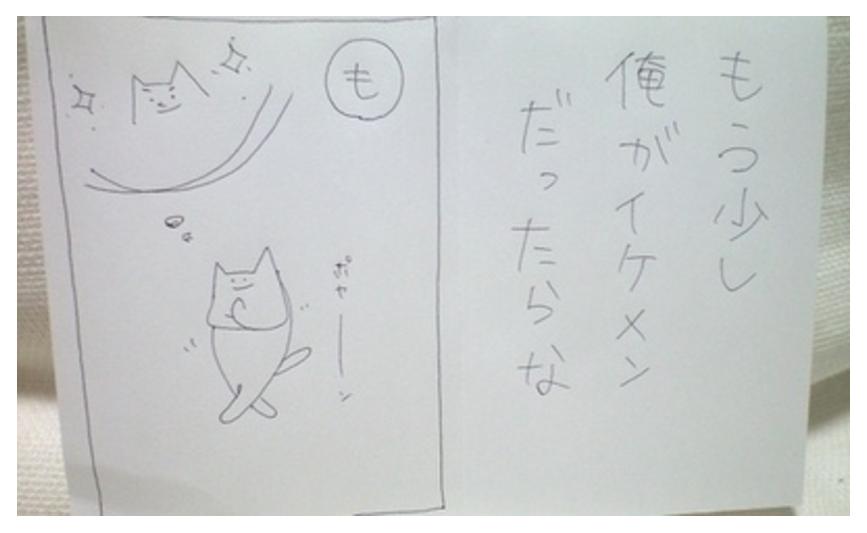
\includegraphics{sample.eps}

\section{脚注を入れる}

脚注\footnote{これが脚注です.}について.

\section{数式を書く}

\begin{thebibliography}{9}
  \bibitem{Knuth}
     結城浩,“プログラマの数学”,ソフトバンク クリエイティブ (2005).
\end{thebibliography}


\end{document}
